% Assignment 3 - Parallel Matrix Multiplication and Optional Vectorisation
% Author: Tomas Santana
% Compile with pdflatex (Overleaf-ready). Upload this file together with the
% tables/ and figures/ folders. Every table and figure referenced here is
% auto-generated by assignment3/scripts/analyze_results.py and
% collect_system_info.py from the raw measurement CSVs.
\documentclass[11pt,a4paper]{article}

\usepackage[T1]{fontenc}
\usepackage[margin=2.5cm]{geometry}
\usepackage{amsmath,amssymb}
\usepackage{booktabs}
\usepackage{graphicx}
\usepackage{pmboxdraw}
\usepackage{microtype}
\usepackage{caption}
\usepackage{float}
\usepackage[section]{placeins}
\usepackage[hidelinks]{hyperref}

\graphicspath{{figures/}}

\title{\textbf{Parallel Matrix Multiplication}\\and Optional Vectorisation\\
\large Assignment 3 --- Big Data, Grado en Ciencia e Ingeniería de Datos, ULPGC}
\author{Tomás Santana Suárez}
\date{Academic year 2026--2027}

\begin{document}
\maketitle

% =====================================================================
\begin{abstract}
\noindent This study asks how the number of threads $p$ affects the kernel
time, speedup and efficiency of a shared-memory dense matrix multiplication,
and when parallel execution helps. The validated cache-blocked kernel of
Assignment 2 is parallelised with OpenMP over row tiles; its sequential
baseline is the \emph{same source file} compiled without OpenMP, so
algorithm, layout, numeric type (float64), inputs and accumulation order are
identical by construction and every parallel result is bit-identical to the
sequential one. On a hybrid Intel i7-14700HX (8 P-cores with SMT + 12
E-cores, 28 logical processors) and $n \in \{400,\dots,4000\}$, with one
warm-up and five measured repetitions per configuration, the speedup is
near-linear up to $p=4$ and peaks at $S \approx 5.4$--$7.8$ for $p=8$--$16$
($E \approx 0.5$--$0.85$); beyond the eight P-cores it stalls, and for
$n \ge 3000$ it \emph{falls} to $S \approx 3.3$--$4.0$ at $p=28$. A probe
experiment shows that the fall is caused by the aggregate per-thread tile
working set overflowing the shared last-level cache: with $256$-wide instead
of $512$-wide tiles, $p=28$ runs $2.8\times$ faster at $n=4000$. The
parallel implementation with $p=1$ costs at most $5\%$ over the sequential
baseline. Two further findings are reported: Windows power management placed
some 1-thread runs on E-cores, slowing the baseline by up to
$\approx 2\times$ and inflating speedups, until it was controlled; and compiler vectorisation (AVX2, verified in the
generated assembly) gives a $2.2$--$2.6\times$ gain that is largely
independent of $p$. Conclusions are scoped to this machine and kernel.
\end{abstract}

% =====================================================================
\section{Introduction and Objective}

Assignments 1 and 2 established a validated triple-loop baseline and showed
that cache blocking reduces the sequential kernel time of $n\times n$
multiplication by more than an order of magnitude at large $n$. All of that
work used a single core of a 28-thread laptop processor. This study measures
what thread-level parallelism adds on top of the best sequential kernel, and
where it stops helping.

\paragraph{Research question.} \emph{How does the thread count $p$ affect
the runtime, speedup and efficiency of a shared-memory, cache-blocked dense
matrix multiplication, and under which conditions (matrix size, thread count,
core type) does parallel execution help?}

\paragraph{Factors and metrics.} Independent factors: thread count
$p \in \{1,2,4,8,12,16,20,24,28,56\}$ and size
$n \in \{400, 1000, 2000, 3000, 4000\}$ ($n$ is the side length of a square
matrix). Dependent metrics: kernel time, speedup
$S(p)=T_{\mathrm{seq}}(n)/T_p(n)$, efficiency $E(p)=S(p)/p$ (all from
\emph{median} times) and peak resident memory. The optional SIMD extension
varies only the compiler vectoriser.

\paragraph{Hypotheses (stated before measuring).}
\textbf{H1:} $S(p)$ is close to $p$ up to the eight performance cores,
because the row tiles are independent and the kernel is compute-bound in
cache. \textbf{H2:} beyond $p=8$ efficiency drops clearly, because further
threads run on SMT siblings or on slower E-cores. \textbf{H3:} for small $n$
the speedup saturates earlier, because a few hundred microseconds of work
cannot amortise thread coordination and there are few row tiles.
\textbf{H4:} AVX2 vectorisation (four doubles per instruction) speeds up the
kernel by $2$--$4\times$, independently of $p$.

% =====================================================================
\section{Background and References}

\subsection{Shared-memory parallelism and its limits}
OpenMP~\cite{openmp52} expresses loop parallelism with compiler directives;
a \texttt{parallel for} region forks a team of threads that share the
iteration space under a chosen schedule and join at an implicit barrier.
Amdahl's law~\cite{amdahl1967} bounds the speedup of a fixed workload by its
serial fraction, and Gustafson~\cite{gustafson1988} notes that the bound
relaxes when the workload grows with the resources. In practice dense
multiplication has a negligible serial fraction, so the binding limits are
hardware resources shared by the threads: memory bandwidth and the
last-level cache. The roofline model~\cite{williams2009} formalises this:
attainable throughput is the minimum of peak compute and memory bandwidth
times arithmetic intensity, so adding cores helps only while the kernel stays
on the compute side of the roof.

\subsection{Blocking, shared caches and hybrid processors}
Cache blocking (tiling)~\cite{lam1991cache,goto2008} keeps a sub-matrix in
fast memory so that each loaded element is reused many times; the right tile
size depends on the cache capacity available \emph{per thread}. On a
multicore chip the last-level cache (L3) is shared, so the effective capacity
per thread falls as threads are added~\cite{hennessy2017}. The test machine
is a hybrid design: performance cores (P-cores) with two hardware threads
each (SMT) and smaller efficiency cores (E-cores). Two threads on one P-core
share its execution units, and an E-core has a lower throughput, so the
logical-processor count overstates the available compute.

\subsection{SIMD vectorisation}
AVX2 registers hold four doubles; a fused multiply--add (FMA) instruction
updates four elements of $C$ per instruction. GCC vectorises loops at
\texttt{-O3} and can be prevented from doing so with
\texttt{-fno-tree-vectorize}~\cite{gccmanual}. Vectorising the innermost
$j$ loop of the $i$-$k$-$j$ order does not reorder the additions into any
single $C_{ij}$, so the result is unchanged under IEEE~754
arithmetic~\cite{ieee754}.

% =====================================================================
\section{Methodology}\label{sec:method}

\subsection{Implementations (custom student code in C)}
\paragraph{Kernel.} The Assignment 2 cache-blocked $i$-$k$-$j$ kernel is
reused with one change: tiles are rectangular, $b_i$ rows $\times$ $b$
columns of the $k$ and $j$ dimensions, with $b=512$ (the Assignment 2 tuned
value). With square $512\times512$ tiles a $2000\times2000$ product has only
four row tiles, too few to feed 28 threads; small row tiles give enough
independent work units while the $k/j$ tiling keeps the sequential cache
behaviour. The loop nest is (row tile, $kk$, $jj$, $i$, $k$, $j$), so every
$C_{ij}$ accumulates its $n$ terms in ascending $k$ order, exactly as in
Assignment 2. Storage is a contiguous row-major \texttt{double} array.

\paragraph{Parallelisation.} One directive,
\texttt{\#pragma omp parallel for schedule(dynamic,1)}, distributes row tiles
among threads. Each tile zeroes and computes only its own rows of $C$, and
$A$ and $B$ are read-only, so no locks or atomics are needed in the
computation (an atomic flag only signals the run-time watchdog). Dynamic
scheduling was chosen because the processor is hybrid: with static, equal
chunks the slowest (E-core) thread would set the completion time.

\paragraph{Equivalent sequential baseline by construction.} The same file is
compiled twice: without \texttt{-fopenmp} the pragmas are ignored and the
code is the sequential baseline (\texttt{tiled\_seq\_vec}); with
\texttt{-fopenmp} it is the parallel implementation (\texttt{tiled\_par\_vec}),
also run with $p=1$ to expose framework overhead. A suffix macro gives the two
objects distinct symbol names so that one harness links both. For the SIMD
extension two more objects are built with \texttt{-fno-tree-vectorize}.
All kernels use \texttt{-O3 -march=native}; no numerical library is linked,
so there are no hidden library threads.

\paragraph{Row-tile tuning.} $b_i$ was chosen before the main experiment
with a short sweep at $n=2000$ (Table~\ref{tab:tune}, $N=3$, diagnostic
only). The sequential kernel prefers tall tiles ($b_i=64$: $692$\,ms), the
parallel one at $p=28$ prefers short ones ($b_i\in\{8,16\}$: $102$\,ms).
$b_i=16$ was selected: it is tied-best in parallel and gives $25$ tiles even
at $n=400$; the cost is a sequential baseline $\approx 20\%$ slower than with
$b_i=64$, which affects $T_{\mathrm{seq}}$ and $T_p$ alike.

% Auto-generated by scripts/analyze_results.py -- do not edit.
\begin{table}[H]
\centering
\small
\caption{Row-tile tuning at $n=2000$: kernel time in ms, median [IQR] of $N=3$ repetitions.}
\label{tab:tune}
\begin{tabular}{rrrrr}
\toprule
Row tile & k/j tile & Row tiles & Sequential & Parallel $p=28$ \\
\midrule
8 & 512 & 250 & 884.6 [8.0] & 101.9 [4.3] \\
16 & 512 & 125 & 827.1 [28.7] & 101.9 [6.0] \\
32 & 512 & 63 & 791.4 [9.3] & 122.7 [6.2] \\
64 & 512 & 32 & 691.6 [4.3] & 112.5 [4.1] \\
\bottomrule
\end{tabular}
\end{table}


\subsection{Inputs}
The Assignment 1 matrices are reused unchanged (\texttt{A\_n.csv},
\texttt{B\_n.csv}; float64, uniform in $[-10,10]$, Mersenne Twister seed 42);
\texttt{scripts/generate\_matrices.py} recreates them bit-identically. $n=400$
replaces a planned $n=500$ because it already exists in the shared dataset.
The same logical inputs feed every method and thread count.

\subsection{Environment and thread placement}\label{sec:env}
Table~\ref{tab:env} is generated by \texttt{collect\_system\_info.py}; the
core topology is read at run time with \texttt{GetLogicalProcessorInformationEx},
not typed by hand. Threads are set per configuration with
\texttt{omp\_set\_num\_threads($p$)} and dynamic adjustment disabled;
$p=56$ is a deliberate $2\times$ oversubscription of the 28 logical
processors. libgomp on Windows does not implement
\texttt{OMP\_PROC\_BIND}/\texttt{OMP\_PLACES} (it reports \emph{``Affinity not
supported on this configuration''}), so placement is controlled with the
Windows API instead (Section~\ref{sec:placement}): the process opts out of
EcoQoS power throttling~\cite{mssetprocinfo}, every 1-thread run (sequential
and $p=1$) is restricted to the 16 P-core logical processors, and runs with
$p\ge2$ may use all 28 logical processors as the OS scheduler decides.

% Auto-generated by scripts/collect_system_info.py -- do not edit.
\begin{table}[H]
\centering
\small
\caption{Benchmarking machine and toolchain.}
\label{tab:env}
\begin{tabular}{lp{0.68\linewidth}}
\toprule
Component & Value \\
\midrule
CPU model & Intel(R) Core(TM) i7-14700HX \\
Core topology & 20 cores / 28 logical: 8 P-cores (16 logical, SMT) + 12 E-cores (12 logical) \\
Last-level cache (L3) & 33 MB \\
Total RAM & 31,7 GB \\
Operating system & Windows 11 (build 10.0.26300) \\
Power plan & High performance (8c5e7fda-e8bf-4a96-9a85-a6e23a8c635c) \\
C compiler & gcc (Rev4, Built by MSYS2 project) 16.2.0 \\
Kernel flags & -O3 -march=native [-fopenmp] [-fno-tree-vectorize] \\
SIMD target & AVX2=1, FMA=1, AVX-512F=0 \\
Threading & OpenMP 202111 (libgomp), dynamic adjustment off, thread count set per run with omp\_set\_num\_threads; OMP\_PROC\_BIND/OMP\_PLACES unsupported by libgomp on this platform; EcoQoS opt-out (ecoqos\_optout=on); 1-thread runs restricted to P-cores, p>=2 runs on all logical processors \\
Library threads & no numerical library linked; OPENBLAS/MKL variables unset \\
Analysis runtime & CPython 3.11.9 \\
\bottomrule
\end{tabular}
\end{table}


\subsection{Timing, repetitions, memory and budgets}
The timer (\texttt{clock\_gettime(CLOCK\_MONOTONIC)}) brackets only the
kernel call. Inputs are loaded and $C$ is allocated outside the timer;
zeroing $C$ is inside it, done per tile by the thread that owns it. Each
configuration runs one warm-up (excluded; it also absorbs the creation of
new OpenMP worker threads) and $N=5$ measured repetitions; the trace of $C$
is logged after every run so the computation cannot be eliminated. The
median is the central statistic and the IQR the variability; $S(p)$ and
$E(p)$ use medians, and the speedup error bars propagate the IQR of $T_p$
with $T_{\mathrm{seq}}$ fixed at its median. Memory is the peak process
working set (resident set), sampled every 5\,ms by a background thread.
Budgets: 120\,s per run (watchdog, logged as \texttt{TIMEOUT} with no time)
and $3\cdot8n^2$ bytes for $A,B,C$ ($366$\,MiB at $n=4000$). Every
configuration completed within budget. Configurations ran in a fixed order
(size, then sequential, then increasing $p$) on AC power with the
\emph{High performance} plan.

\subsection{Correctness}
A gate of 332 automated checks runs before any benchmark and aborts on
failure: $A\times I=A$ and $A\times 0=0$ for $n\in\{1,2,4,8,16\}$; a known
$2\times2$ product; agreement with an independent $k$-$i$-$j$ reference for
$n\in\{1,2,4,8,16,17,33,100\}$, with default tiles and with tiny tiles
($3\times8$) that exercise every remainder path; and \textbf{bitwise
equality} (\texttt{memcmp}) of every parallel result with the sequential one
for $p\in\{1,2,4,28,56\}$, including $p$ larger than the number of tiles.
The output buffer is filled with garbage before each test, so a kernel that
forgot to zero $C$ would fail. Tolerances are $\epsilon_{\mathrm{abs}} =
\epsilon_{\mathrm{rel}} = 10^{-9}$ as in Assignment 2. Bitwise equality is
the strongest available evidence of race freedom: any lost or duplicated
update would change bits. During the benchmark every parallel result was
again compared bitwise with the sequential result of the same input (50/50
identical), and an external NumPy check at $n=1000$, $p=28$ gave
$\max|C-C_{\mathrm{NumPy}}| = 1.4\times10^{-11}$.

% =====================================================================
\section{Results}\label{sec:results}

\subsection{Thread scaling}
Table~\ref{tab:time} lists every median and IQR; Figure~\ref{fig:time} shows
them against $p$, and Table~\ref{tab:speedup} with
Figure~\ref{fig:speedup} gives speedup and efficiency.

% Auto-generated by scripts/analyze_results.py -- do not edit.
\begin{table}[H]
\centering
\small
\caption{Kernel execution time in ms, median [IQR] of $N=5$ measured repetitions (1 warm-up excluded). Sequential baseline and parallel implementation with $p$ threads.}
\label{tab:time}
\begin{tabular}{lrrrrr}
\toprule
Configuration & $n=400$ & $n=1000$ & $n=2000$ & $n=3000$ & $n=4000$ \\
\midrule
Sequential & 4.6 [0.2] & 86.1 [3.5] & 888.5 [45.7] & 3{,}065 [64] & 7{,}566 [339] \\
\midrule
Parallel $p=1$ & 4.6 [0.1] & 90.4 [6.4] & 889.0 [18.8] & 2{,}946 [124] & 7{,}670 [151] \\
Parallel $p=2$ & 2.4 [0.2] & 47.3 [2.1] & 427.5 [6.6] & 1{,}463 [8] & 3{,}629 [57] \\
Parallel $p=4$ & 1.3 [0.1] & 24.9 [0.6] & 227.4 [0.7] & 760.8 [5.3] & 1{,}968 [113] \\
Parallel $p=8$ & 0.9 [0.1] & 14.6 [0.5] & 128.5 [2.2] & 449.7 [16.5] & 1{,}294 [460] \\
Parallel $p=12$ & 1.0 [0.2] & 13.2 [1.5] & 124.5 [8.8] & 466.5 [10.9] & 1{,}574 [28] \\
Parallel $p=16$ & 0.9 [0.1] & 11.0 [0.6] & 127.1 [3.2] & 509.3 [20.4] & 1{,}550 [43] \\
Parallel $p=20$ & 1.5 [0.2] & 12.8 [2.9] & 139.1 [11.5] & 726.9 [10.1] & 2{,}050 [195] \\
Parallel $p=24$ & 0.9 [0.1] & 13.6 [1.1] & 136.1 [5.5] & 807.4 [18.7] & 2{,}156 [26] \\
Parallel $p=28$ & 0.9 [0.1] & 12.7 [1.8] & 127.2 [5.9] & 772.4 [53.8] & 2{,}278 [226] \\
Parallel $p=56$ & 0.9 [0.1] & 11.7 [1.8] & 143.2 [2.7] & 778.1 [16.5] & 2{,}213 [100] \\
\bottomrule
\end{tabular}
\end{table}


\begin{figure}[H]
\centering
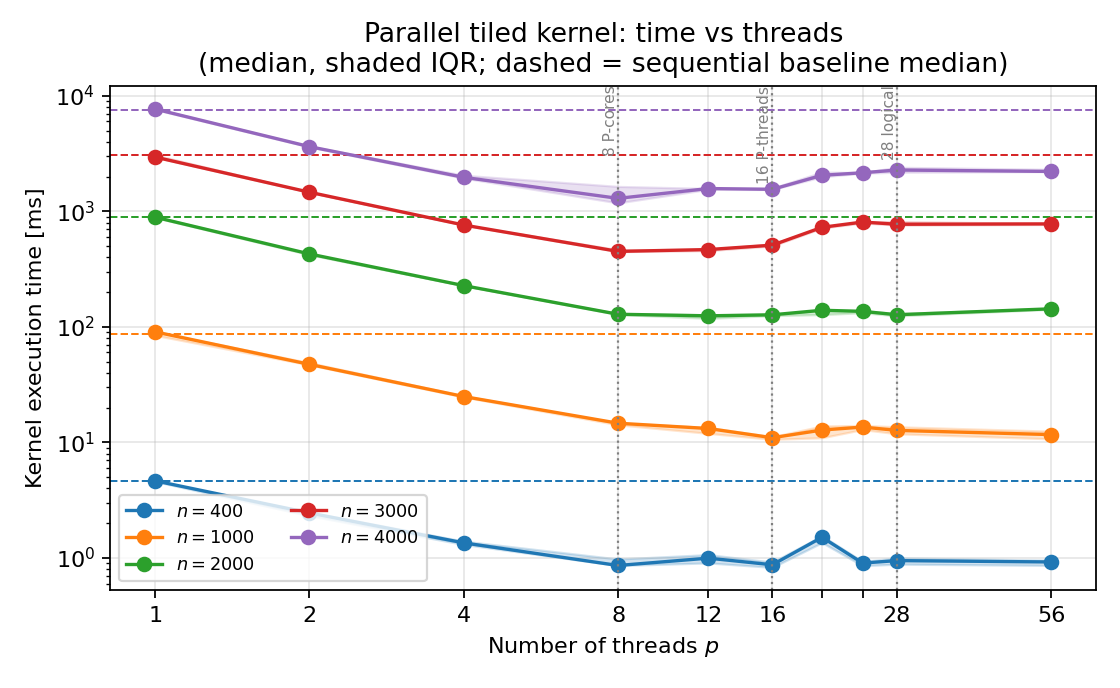
\includegraphics[width=0.82\linewidth]{fig_time_vs_threads.png}
\caption{Kernel time of the parallel implementation versus $p$ (log--log),
median with shaded IQR; dashed lines are the sequential baseline medians.
Dotted guides mark the 8 P-cores, their 16 hardware threads and the 28
logical processors.}
\label{fig:time}
\end{figure}

% Auto-generated by scripts/analyze_results.py -- do not edit.
\begin{table}[H]
\centering
\small
\caption{Speedup $S(p)=T_{\mathrm{seq}}(n)/T_p(n)$ and, in parentheses, efficiency $E(p)=S(p)/p$, both computed from median times.}
\label{tab:speedup}
\begin{tabular}{lccccc}
\toprule
$p$ & $n=400$ & $n=1000$ & $n=2000$ & $n=3000$ & $n=4000$ \\
\midrule
1 & 0.99 (0.99) & 0.95 (0.95) & 1.00 (1.00) & 1.04 (1.04) & 0.99 (0.99) \\
2 & 1.88 (0.94) & 1.82 (0.91) & 2.08 (1.04) & 2.10 (1.05) & 2.09 (1.04) \\
4 & 3.41 (0.85) & 3.45 (0.86) & 3.91 (0.98) & 4.03 (1.01) & 3.84 (0.96) \\
8 & 5.35 (0.67) & 5.88 (0.73) & 6.92 (0.86) & 6.81 (0.85) & 5.85 (0.73) \\
12 & 4.62 (0.39) & 6.53 (0.54) & 7.14 (0.59) & 6.57 (0.55) & 4.81 (0.40) \\
16 & 5.28 (0.33) & 7.85 (0.49) & 6.99 (0.44) & 6.02 (0.38) & 4.88 (0.31) \\
20 & 3.05 (0.15) & 6.73 (0.34) & 6.39 (0.32) & 4.22 (0.21) & 3.69 (0.18) \\
24 & 5.10 (0.21) & 6.34 (0.26) & 6.53 (0.27) & 3.80 (0.16) & 3.51 (0.15) \\
28 & 4.86 (0.17) & 6.78 (0.24) & 6.98 (0.25) & 3.97 (0.14) & 3.32 (0.12) \\
56 & 4.99 (0.09) & 7.37 (0.13) & 6.20 (0.11) & 3.94 (0.07) & 3.42 (0.06) \\
\bottomrule
\end{tabular}
\end{table}


\begin{figure}[H]
\centering
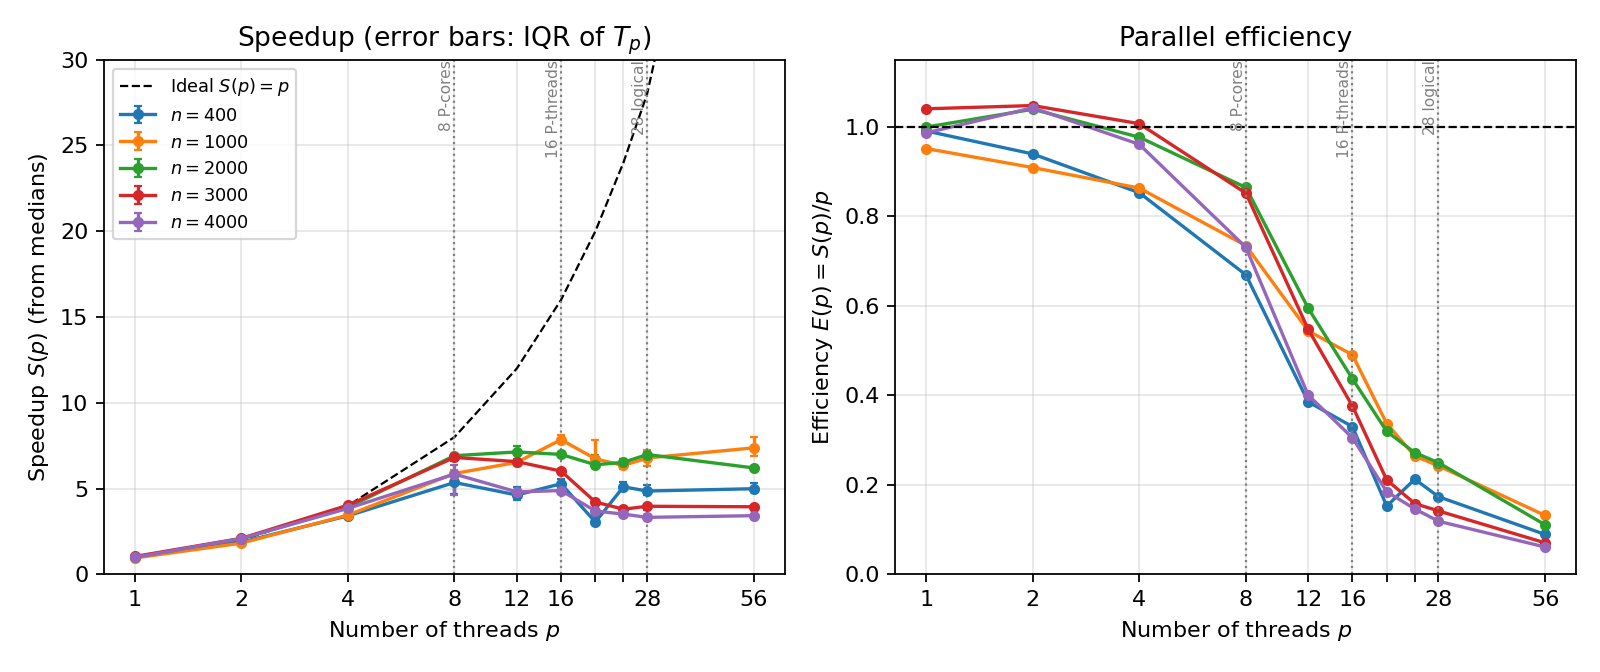
\includegraphics[width=\linewidth]{fig_speedup_efficiency.png}
\caption{Speedup (left, with ideal $S=p$) and efficiency (right) from median
times. Error bars: range of $S$ induced by the IQR of $T_p$.}
\label{fig:speedup}
\end{figure}

Three regimes are visible. (i) $p\le4$: near-linear scaling at every size
($S(4)=3.4$--$4.0$, $E\ge0.85$). (ii) $4<p\le16$: diminishing returns; the
best speedup per size is $5.35$ ($n=400$, $p=8$), $7.85$ ($n=1000$, $p=16$),
$7.14$ ($n=2000$, $p=12$), $6.81$ ($n=3000$, $p=8$) and $5.85$ ($n=4000$,
$p=8$). (iii) $p>16$: for $n\le2000$ the time is flat within a few percent,
but for $n\ge3000$ it \emph{increases}: at $n=4000$ the kernel takes
$1.29$\,s with 8 threads and $2.28$\,s with 28. The parallel build with
$p=1$ is within $-4\%$ to $+5\%$ of the sequential baseline. Oversubscription
($p=56$) is never better than the best $p\le28$, and never much worse
than $p=28$.

\subsection{Memory}
% Auto-generated by scripts/analyze_results.py -- do not edit.
\begin{table}[H]
\centering
\small
\caption{Peak process working set (RSS) in MB, median of the measured repetitions, versus the theoretical storage of $A$, $B$ and $C$ ($3\cdot 8n^2$ bytes).}
\label{tab:memory}
\begin{tabular}{lrrrrr}
\toprule
Configuration & $n=400$ & $n=1000$ & $n=2000$ & $n=3000$ & $n=4000$ \\
\midrule
Theoretical $A,B,C$ & 3.7 & 22.9 & 91.6 & 206.0 & 366.2 \\
\midrule
Sequential & 10.2 & 29.4 & 98.1 & 212.5 & 372.7 \\
Parallel $p=1$ & 11.4 & 37.1 & 128.6 & 281.2 & 494.8 \\
Parallel $p=28$ & 11.0 & 36.6 & 128.2 & 280.7 & 494.4 \\
Parallel $p=56$ & 11.4 & 37.1 & 128.6 & 281.2 & 494.9 \\
\bottomrule
\end{tabular}
\end{table}

The peak working set does not depend on $p$: at every size the values for
$p=1$, $28$ and $56$ agree within $0.5$\,MB, so per-thread stacks and the
OpenMP runtime are negligible. The sequential baseline is
$6$--$7$\,MB above the theoretical storage of $A,B,C$; the parallel rows are
exactly one matrix larger ($122.1$\,MB $=8\cdot4000^2$ bytes at $n=4000$)
because, after the sequential run, the harness keeps a copy of its result
for the bitwise cross-check. That buffer belongs to the measurement harness,
not to the parallel kernel.

\subsection{SIMD extension}
% Auto-generated by scripts/analyze_results.py -- do not edit.
\begin{table}[H]
\centering
\small
\caption{SIMD extension: kernel time in ms, median [IQR] ($N=5$), of the non-vectorised (\texttt{-fno-tree-vectorize}) and vectorised builds of the same source, at $p=1$ (sequential) and $p=8$. Gain $=T_{\mathrm{novec}}/T_{\mathrm{vec}}$ (medians).}
\label{tab:simd}
\begin{tabular}{rrrcrrc}
\toprule
 & \multicolumn{3}{c}{Sequential ($p=1$)} & \multicolumn{3}{c}{Parallel ($p=8$)} \\
\cmidrule(lr){2-4}\cmidrule(lr){5-7}
$n$ & novec & vec & gain & novec & vec & gain \\
\midrule
1000 & 237.4 [2.3] & 89.9 [2.8] & 2.64 & 34.5 [2.2] & 14.6 [1.0] & 2.35 \\
2000 & 2{,}120 [32] & 897.7 [18.4] & 2.36 & 302.4 [17.3] & 135.6 [10.3] & 2.23 \\
3000 & 6{,}889 [212] & 3{,}041 [52] & 2.27 & 1{,}047 [24] & 478.4 [17.8] & 2.19 \\
\bottomrule
\end{tabular}
\end{table}


\begin{figure}[H]
\centering
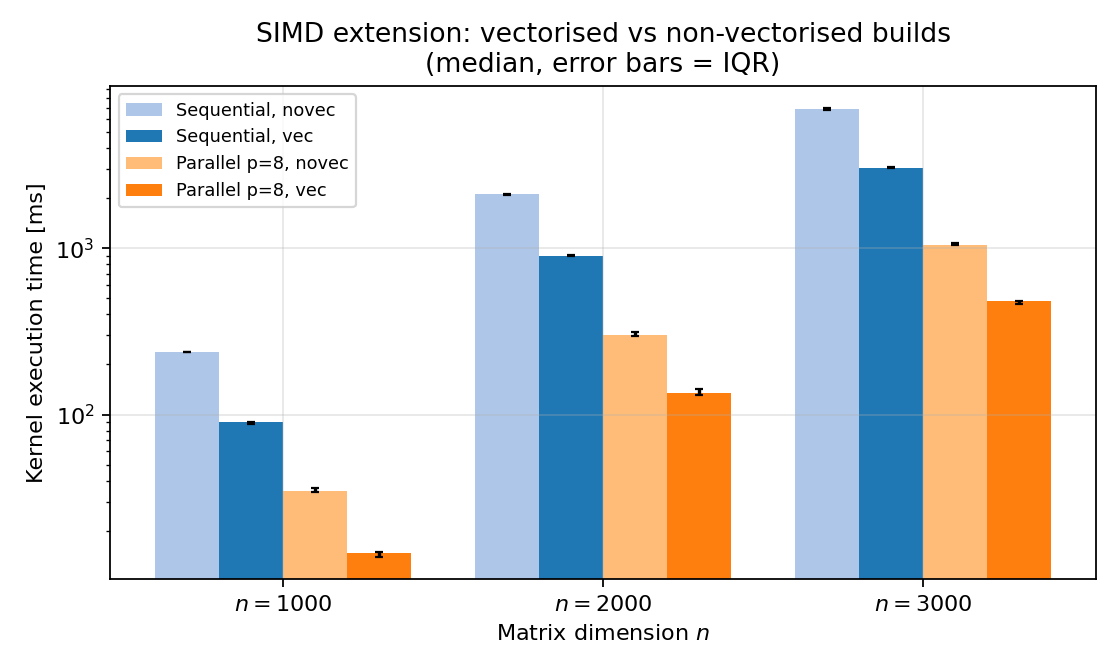
\includegraphics[width=0.72\linewidth]{fig_simd.png}
\caption{Vectorised versus non-vectorised builds at $p=1$ and $p=8$
(median, IQR error bars).}
\label{fig:simd}
\end{figure}

Evidence that vectorisation occurs, and only where intended: the GCC
report (\texttt{-fopt-info-vec-optimized}) states for the innermost $j$
loop \emph{``loop vectorized using 32 byte vectors''} in both vec objects and
reports nothing for the novec objects; \texttt{objdump} finds the packed
256-bit FMA \texttt{vfmadd213pd (\dots),\%ymm1,\%ymm0} in the inner loop of
the vec objects and only the scalar \texttt{vfmadd\dots sd} in the novec
objects (\texttt{data/results/simd\_evidence.csv}). All four builds produce
bit-identical results. Vectorisation gives $2.27$--$2.64\times$ at $p=1$ and
$2.19$--$2.35\times$ at $p=8$ ($p=8$ was the best or near-best thread count
for $n\ge2000$ in the main experiment, and stays within the 8 P-cores).

\subsection{Placement diagnostic and probe experiments}\label{sec:placement}
A first complete run of the thread sweep without placement control produced
1-thread times inconsistent with cubic growth and with the tuning run of the
same kernel ($1.75$\,s at $n=2000$ against $0.77$\,s; $6.38$\,s at $n=3000$
against $6.55$\,s at $n=4000$) and speedups up to $11.5$.
Table~\ref{tab:placement} isolates the cause with three policies; that run
is kept in \texttt{data/results/superseded/} and is not used in any other
table.

% Auto-generated by scripts/analyze_results.py -- do not edit.
\begin{table}[H]
\centering
\small
\caption{Placement diagnostic: 1-thread kernel time in ms, median [IQR] of $N=3$ repetitions (row tile 32), for the sequential baseline and the parallel build with $p=1$, under three Windows placement policies. Both columns execute identical work.}
\label{tab:placement}
\begin{tabular}{lrrrr}
\toprule
 & \multicolumn{2}{c}{$n=2000$} & \multicolumn{2}{c}{$n=3000$} \\
\cmidrule(lr){2-3}\cmidrule(lr){4-5}
Policy & Seq. & Par. $p=1$ & Seq. & Par. $p=1$ \\
\midrule
Windows default (EcoQoS on, any core) & 825.3 [4.0] & 829.9 [26.3] & 6{,}028 [277] & 2{,}763 [37] \\
EcoQoS opt-out, any core & 744.9 [18.8] & 761.9 [29.8] & 2{,}878 [144] & 2{,}769 [33] \\
EcoQoS opt-out, P-cores only & 766.1 [31.1] & 812.4 [12.0] & 2{,}652 [22] & 2{,}589 [16] \\
\bottomrule
\end{tabular}
\end{table}


To test the explanation of the large-$n$ slowdown (Section~\ref{sec:disc}),
Table~\ref{tab:probe} varies the tile shape at $n=4000$ ($N=3$, diagnostic).

% Auto-generated by scripts/analyze_results.py -- do not edit.
\begin{table}[H]
\centering
\small
\caption{Row-tile probe of the large-$n$ slowdown at $n=4000$: kernel time in ms, median [IQR] of $N=3$ repetitions.}
\label{tab:probe}
\begin{tabular}{rrrrrr}
\toprule
Row tile & k/j tile & Row tiles & Sequential & Parallel $p=8$ & Parallel $p=28$ \\
\midrule
16 & 512 & 250 & 7{,}694 [35] & 1{,}170 [49] & 1{,}867 [336] \\
64 & 512 & 63 & 6{,}452 [114] & 1{,}111 [92] & 1{,}675 [88] \\
128 & 512 & 32 & 6{,}285 [152] & 1{,}125 [75] & 1{,}771 [102] \\
16 & 256 & 250 & 5{,}648 [103] & 964.1 [24.2] & 669.3 [17.3] \\
16 & 128 & 250 & 6{,}025 [254] & 887.8 [13.3] & 680.9 [8.5] \\
\bottomrule
\end{tabular}
\end{table}


% =====================================================================
\section{Discussion}\label{sec:disc}

\subsection{When does parallel execution help?}
Parallelism pays off at every tested size: even at $n=400$ (a $4.6$\,ms
kernel) eight threads give $5.35\times$, and from $n=1000$ the best
configuration is $5.9$--$7.9\times$ faster than the identical sequential
baseline, itself the fastest kernel of Assignment 2. The useful range, however, ends near the number of
P-cores: the best $p$ is 8--16 at every size. \textbf{H1} is confirmed up to
$p=4$ ($E\ge0.85$) and only partially at $p=8$ ($E=0.67$--$0.86$).
\textbf{H2} is confirmed and stronger than expected: efficiency collapses
beyond $p=8$, and for large $n$ adding threads makes the kernel slower.

\subsection{Why scaling stops: P-cores, SMT and E-cores}
Up to $p=8$ the scheduler can give every thread its own P-core. Threads 9--16
must share P-cores through SMT, which adds little throughput to an FMA-bound
inner loop, and threads 17--28 land on E-cores. With dynamic scheduling the
slow cores do not delay the others---they simply take fewer tiles---so for
$n\le2000$ the curve is flat rather than falling. This explains the
plateau but not the \emph{decline} at $n\ge3000$.

\subsection{Why large matrices get slower: shared-cache capacity}
Each thread works on its own row tile, but it sweeps \emph{all} of $B$ in
$512\times512$ panels of $2$\,MiB. Threads drift apart under dynamic
scheduling, so at any moment they touch different $B$ panels: the aggregate
working set is about $p\times2$\,MiB, which exceeds the $33$\,MB L3 beyond
roughly 16 threads. For $n=2000$ the whole $B$ ($30.5$\,MiB) still fits in
L3, so threads hit the same cached data regardless of position; for
$n=3000$ ($68.7$\,MiB) and $n=4000$ ($122$\,MiB) it does not, and the extra
threads turn L3 hits into DRAM traffic. This hypothesis predicts that
shrinking the $k/j$ tile should remove the decline, while changing the row
tile should not. Table~\ref{tab:probe} confirms both predictions: taller row
tiles ($b_i=64,128$) leave $p=28$ at $1.7$--$1.8$\,s, whereas $b=256$
($28\times0.5$\,MiB $=14$\,MiB, within L3) brings $p=28$ to $0.67$\,s,
$2.8\times$ faster than with $b=512$ and now faster than $p=8$ ($0.96$\,s),
for a speedup of $8.4$ against the matching sequential run. The block size
tuned for one core in Assignment 2 is therefore not the right block size
for many cores sharing a cache, which is consistent with blocking
theory~\cite{lam1991cache,goto2008}. The probe is a small diagnostic
($N=3$, one size) and does not replace a full re-tuning.

\subsection{Small matrices and overhead (H3)}
\textbf{H3} is confirmed: at $n=400$ the speedup saturates at $\approx5$ by
$p=8$ and is noisy above (e.g.\ $S(20)=3.05$ against $S(24)=5.10$). A
sub-millisecond parallel run is sensitive to the time it takes to wake 20+
threads, and 25 row tiles cannot be balanced across 20--28 threads of mixed
speed. The cost of the framework itself is small: $T_p$ at $p=1$ is within
$-4\%$/$+5\%$ of $T_{\mathrm{seq}}$, comparable to the run-to-run IQR.

\subsection{Is the slight superlinearity at $p=2$ real?}
$S(2)=2.08$--$2.10$ for $n\ge2000$ ($E\approx1.04$). The excess ($4$--$5\%$)
is the same size as the sequential IQR (e.g.\ $64$\,ms of $3065$\,ms at
$n=3000$, $340$\,ms of $7566$\,ms at $n=4000$) and as the $p=1$ versus
sequential difference, so the data do not support a claim of genuine
superlinear speedup. A plausible but untested contributor is that two threads
use two private L2 caches instead of one.

\subsection{Placement anomaly}
Under the Windows default the sequential baseline at $n=3000$ took
$6.0$\,s while the identical $p=1$ run took $2.8$\,s
(Table~\ref{tab:placement}): with EcoQoS active, a process that is not in
the foreground can be steered to E-cores, and the effect hit some 1-thread
runs but not others. Opting out of EcoQoS alone reduced the gap; restricting
1-thread runs to P-cores closed it ($2.65$ vs $2.59$\,s). Without this
control, speedups computed against an E-core baseline would have been
inflated by up to $\approx2\times$. The policy makes $T_{\mathrm{seq}}$ the
time on the fastest core type, which is the conservative choice for $S(p)$.

\subsection{SIMD (H4)}
\textbf{H4} is confirmed: vectorisation gives $2.2$--$2.6\times$, inside the
predicted $2$--$4\times$ and below the 4-lane maximum because the
non-vectorised build already uses scalar FMA and both builds load $B$ and
store $C$ from the same cache levels. The gain is slightly lower at $p=8$
($2.19$--$2.35$) than at $p=1$ ($2.27$--$2.64$), consistent with the threads
starting to share memory bandwidth. Vectorisation and threading multiply
almost independently: at $n=3000$, $p=8$ with vectorisation is $14.4\times$
faster than the sequential non-vectorised build.

\subsection{Limitations}
(i) One laptop, one compiler and one kernel; the numbers do not generalise to
other microarchitectures or to library BLAS. (ii) OpenMP affinity is
unavailable, so for $p\ge2$ thread placement is decided by Windows and
varies between runs (e.g.\ the $460$\,ms IQR at $n=4000$, $p=8$).
(iii) Configurations ran in a fixed order, so slow thermal drift cannot be
excluded. (iv) No hardware counters were collected; the cache-capacity
explanation rests on the controlled probe and on working-set arithmetic,
not on measured miss rates. (v) Tuning and probe experiments use $N=3$.
(vi) The memory metric is process-wide and includes harness buffers.

% =====================================================================
\section{Conclusions}

Within the tested scope (C + OpenMP, float64, cache-blocked $i$-$k$-$j$,
$n\le4000$, one hybrid 28-thread laptop CPU):

\begin{enumerate}
\item Parallel execution helps at every tested size. With $b=512$ tiles the
best speedup over an identical sequential baseline is $5.4$--$7.8\times$,
reached with 8--16 threads, i.e.\ about one thread per P-core.
\item Scaling is near-linear up to $p=4$; past the eight P-cores efficiency
collapses, and for $n\ge3000$ more threads are slower ($S$ falls from
$5.9$--$6.8$ at $p=8$ to $3.3$--$4.0$ at $p=28$). A probe isolates the cause
as shared-L3 capacity: halving the $k/j$ tile makes 28 threads
$2.8\times$ faster at $n=4000$. Block sizes must be tuned for the thread
count, not only for one core.
\item OpenMP overhead is negligible ($p=1$ within $\pm5\%$ of the
sequential baseline), memory is independent of $p$, and parallel results are
bit-identical to sequential ones.
\item On a hybrid CPU the OS placement policy is part of the experiment:
uncontrolled, it slowed 1-thread baselines by up to $2\times$ and inflated
the speedups accordingly.
\item Compiler vectorisation (AVX2) adds $2.2$--$2.6\times$ on top of, and
largely independently of, threading.
\end{enumerate}

Open questions for Assignment 4: a full re-tuning of $(b_i, b)$ as a
function of $p$; whether distributed workers, each with its own cache and
memory bandwidth, avoid the shared-cache limit observed here; and how
communication costs compare with the $\approx0.1$--$2$\,s kernels measured
in this study.

% =====================================================================
\begin{thebibliography}{10}

\bibitem{openmp52}
OpenMP Architecture Review Board, \emph{OpenMP Application Programming
Interface, Version 5.2}, Nov. 2021. [Online]. Available:
\url{https://www.openmp.org/specifications/}

\bibitem{amdahl1967}
G. M. Amdahl, ``Validity of the single processor approach to achieving large
scale computing capabilities,'' in \emph{Proc. AFIPS Spring Joint Computer
Conf.}, 1967, pp. 483--485.

\bibitem{gustafson1988}
J. L. Gustafson, ``Reevaluating Amdahl's law,'' \emph{Commun. ACM}, vol. 31,
no. 5, pp. 532--533, 1988.

\bibitem{williams2009}
S. Williams, A. Waterman, and D. Patterson, ``Roofline: An insightful visual
performance model for multicore architectures,'' \emph{Commun. ACM}, vol. 52,
no. 4, pp. 65--76, 2009.

\bibitem{lam1991cache}
M. S. Lam, E. E. Rothberg, and M. E. Wolf, ``The cache performance and
optimizations of blocked algorithms,'' in \emph{Proc. 4th Int. Conf.
Architectural Support for Programming Languages and Operating Systems
(ASPLOS-IV)}, 1991, pp. 63--74.

\bibitem{goto2008}
K. Goto and R. A. van de Geijn, ``Anatomy of high-performance matrix
multiplication,'' \emph{ACM Trans. Math. Softw.}, vol. 34, no. 3, art. 12,
2008.

\bibitem{hennessy2017}
J. L. Hennessy and D. A. Patterson, \emph{Computer Architecture: A
Quantitative Approach}, 6th ed. Cambridge, MA, USA: Morgan Kaufmann, 2017.

\bibitem{gccmanual}
Free Software Foundation, ``Options that control optimization,'' in
\emph{Using the GNU Compiler Collection (GCC)}. [Online]. Available:
\url{https://gcc.gnu.org/onlinedocs/gcc/Optimize-Options.html}

\bibitem{mssetprocinfo}
Microsoft, ``SetProcessInformation function (processthreadsapi.h),''
\emph{Microsoft Learn}. [Online]. Available:
\url{https://learn.microsoft.com/en-us/windows/win32/api/processthreadsapi/nf-processthreadsapi-setprocessinformation}

\bibitem{ieee754}
IEEE Standard for Floating-Point Arithmetic, IEEE Std 754-2019.

\end{thebibliography}

% =====================================================================
\section*{References and Materials}

\subsection*{Repository structure}
\begin{verbatim}
assignment3/
├── src/c/            tiled kernel (4 builds), harness, validation,
│                     system/affinity helpers
├── scripts/          build, generator, NumPy check, system info, analysis
├── data/results/     raw CSVs, cross-check logs, vectorisation evidence,
│                     placement diagnostic, superseded first run
├── report/           this report, generated figures and tables
└── README.md         build/run instructions and protocol
\end{verbatim}

\subsection*{Reproducibility}
Build and run commands, the CSV schema and the full configuration are in
\texttt{assignment3/README.md}. The reused Assignment 1 dataset is
regenerated bit-identically by \texttt{scripts/generate\_matrices.py}; every
raw measurement is published in \texttt{data/results/} and every table and
figure is regenerated by \texttt{scripts/analyze\_results.py} and
\texttt{scripts/collect\_system\_info.py}. Source code and data:
\url{https://github.com/TemiArtemi/MatrixMultiplicationBigData}.

\subsection*{Generative AI disclosure statement}
The author used a large language-model coding assistant (Claude Code,
Anthropic) for code scaffolding, experiment-planning discussions, analysis
scripting and language editing of this report. All implementations,
measurement protocols and analysis scripts were reviewed, compiled, executed
and validated on the machine described in Table~\ref{tab:env}; every
reported number originates from the raw measurement files in this package.
The author takes full responsibility for the code, the data, the cited
references and the conclusions.

\end{document}
